\chapter{Dashboardvisualisierung} % 5-6 Seiten? 
\label{ch:auswahl}
Im vorherigen Kapitel wurde beschrieben, wie Nutzerdaten erfasst werden können. Hierfür wurden relevante KPIs für das Bildungsportal definiert und verschiedene Methoden der Datenerhebung sowie deren DSGVO-konforme Umsetzung erläutert. Um die gesammelten Daten strukturiert und übersichtlich darzustellen und der Professur für Geschichtsdidaktik eine fundierte Grundlage für datenbasierte Erkenntnisse zu bieten, sollen die KPIs visuell auf einem Dashboard aufbereitet werden. Dazu werden zunächst die eigenen Anforderungen an das Dashboard aufgezählt. Anschließend werden die Struktur sowie der Aufbau des Dashboards anhand der Anforderungen aus Unterkapitel~\ref{sssec:usability} festgelegt. Außerdem werden geeignete Visualisierungsmethoden für die KPIs definiert. Abschließend wird Grafana als Visualisierungslösung vorgestellt. Hierbei wird auf das Unterkapitel~\ref{sssec:technfunk} Bezug genommen und beschrieben wie die technisch-funktionalen Anforderungen in Grafana realisiert werden können.

\section{Anforderungen an das Dashboard}
\label{sec:anforderungen}
\subsection{Technisch-funktionale Anforderungen}
\label{sssec:technfunk}
Die technisch-funktionalen Anforderungen sollen bei der Auswahl einer Dashboard Lösung Orientierung geben. Welche Funktionen ein Dashboard bereitstellen muss und welche technologischen Rahmenbedingungen erfüllt sein müssen, um eine effiziente Nutzung zusammen mit Matomo zu gewährleisten. Diese Anforderungen sind: 
\begin{itemize}
    \item \textbf{Datenintegration und Aggregation:} Das Dashboard Tool soll in der Lage sein, Daten aus Matomo oder alternativ direkt aus der Datenbank zu beziehen und zu aggregieren. Außerdem sollen die per Webanalysetool erfassten Daten automatisch aktualisiert werden. Entweder in definierten Intervallen oder in Echtzeit.
    \item \textbf{Filtermöglichkeiten} Es soll die Möglichkeit geboten werden, die Daten nach einem Datum, Zeitraum und Benutzergruppen zu filtern.
    \item \textbf{Sicherheit und Zugriffskontrolle:} Es muss sichergestellt werden, dass nur authentifizierte Benutzer zugriff auf das Dashboard haben. Außerdem soll eine Rollenbasierte Zugriffskontrolle (engl. Roll based Access Controll (RBAC)) implementiert werden.
\end{itemize}

\subsection{Usability- und Design Anforderungen}
\label{sssec:usability}
Neben technischen Aspekten ist die Benutzerfreundlichkeit des Dashboards nicht zu vernachlässigen. Gerade weil das Dashboard in erster Linie von Nicht-Informatikern verwendet wird, ist eine intuitive Gestaltung wichtig, um einen guten Überblick und eine schnelle Orientierung zu ermöglichen. Wichtige Anforderungen sind hierbei:
\begin{itemize}
    \item \textbf{Anordnung der Inhalte:} Die KPIs sollten so dargestellt werden, dass verwandte Indikatoren auch im Dashboard nebeneinander zu finden sind.
    \item \textbf{Konsistenz in Farben \& Darstellungen:} Ein einheitliches Farbschema soll die Orientierung erleichtern. Es soll dazu dienen positive (z.B. in grün) und negative (z.B. in rot) Trends einer KPI auf dem ersten Blick zu erkennen. Ebenfalls sollen konsistente Darstellungen für identische KPIs verwendet werden.
    \item \textbf{Interaktive Elemente:} (*genauer) Für KPIs, für welche es sinnvoll ist, sollte das Dashboard eine Drill-Down-Funktion bieten, um detailliertere Analysen zu ermöglichen.
\end{itemize}

\section{Struktur und Aufbau des Dashboards}
Bei der Gestaltung eines Dashboards ist es sinnvoll, verwandte KPIs zu gruppieren, um eine klare Struktur und eine bessere Übersichtlichkeit zu gewährleisten. Besonders bei einer großen Anzahl an Kennzahlen hilft diese Form der Gruppierung dabei, die relevanten Informationen gezielt darzustellen, ohne den Gesamtüberblick zu verlieren. [vlg. Hassler, 2019, Kap. 14.3]

Ebenso kann laut Stephen Few die Möglichkeit zur Navigation zwischen unterschiedlichen Dashboardseiten (engl. Screens) eine sinnvolle Funktion sein. Die Aufteilung der KPIs in solche Screens ist allerdings nur dann sinnvoll, wenn dadurch keine Daten fragmentiert werden, welche eigentlich zusammenhängend betrachtet werden sollten. Andernfalls kann eine solche Aufteilung die Effizienz eines Dashboards erheblich einschränken, da zusammengehörige Informationen schwerer in einem sinnvollen Kontext betrachtet werden können. [vlg. Few, 2006, Kap. 3.1.1]

Auch die Notwendigkeit, innerhalb eines Dashboards vertikal oder horizontal zu scrollen, kann die Übersichtlichkeit und Effizienz beeinträchtigen. Laut Few führt dies dazu, dass Nutzer nicht auf einen Blick alle wichtigen Daten erfassen können und häufig nicht bemerken, dass sich weitere relevante Informationen außerhalb des sichtbaren Bereichs befinden. Elemente, die nicht sofort sichtbar sind, werden oft als weniger wichtig wahrgenommen oder gar übersehen, was die Effektivität eines Dashboards erheblich einschränken kann. [ vlg.Few, 2006, Kap. 3.1.1]

Für das Bildungsportal evaschiffmann.de ist es daher sinnvoll, die KPIs auf dedizierten Dashboard-Seiten darzustellen, da diese jeweils demselben Kontext dienen und somit das scrollen vermieden werden kann, welches ohne eine solche Aufteilung auf Grund der Menge unumgänglich wäre. Die KPIs wurden in Kapitel~\ref{sec:kpis} bereits entsprechend für die einzelnen Webseiten des Bildungsportals definiert. Diese Struktur ermöglicht eine gezielte Analyse der verschiedenen Bereiche, weshalb das Dashboard ebenso aufgebaut wird.

\subsection{Anordnung der Elemente}
Um nun die KPIs der jeweiligen Dashboardseiten so anzuordnen, dass Indikatoren, welche dem selben Kontext dienen nah bei einander angezeigt werden, empfiehlt sich eine Gruppierung nach Untersuchungsthema [vlg. Hassler, 2019, Kap. 14.3.1]. Um eine solche Gruppierung zu realisieren, ist es sinnvoll das Dashboard einzuteilen und die einzelnen KPIs an eine Dimension zu binden. Hierzu gibt folgendes Modell in Abbildung ~\ref{fig:dimensionen} auskunft:

\begin{figure}[h]
    \centering
    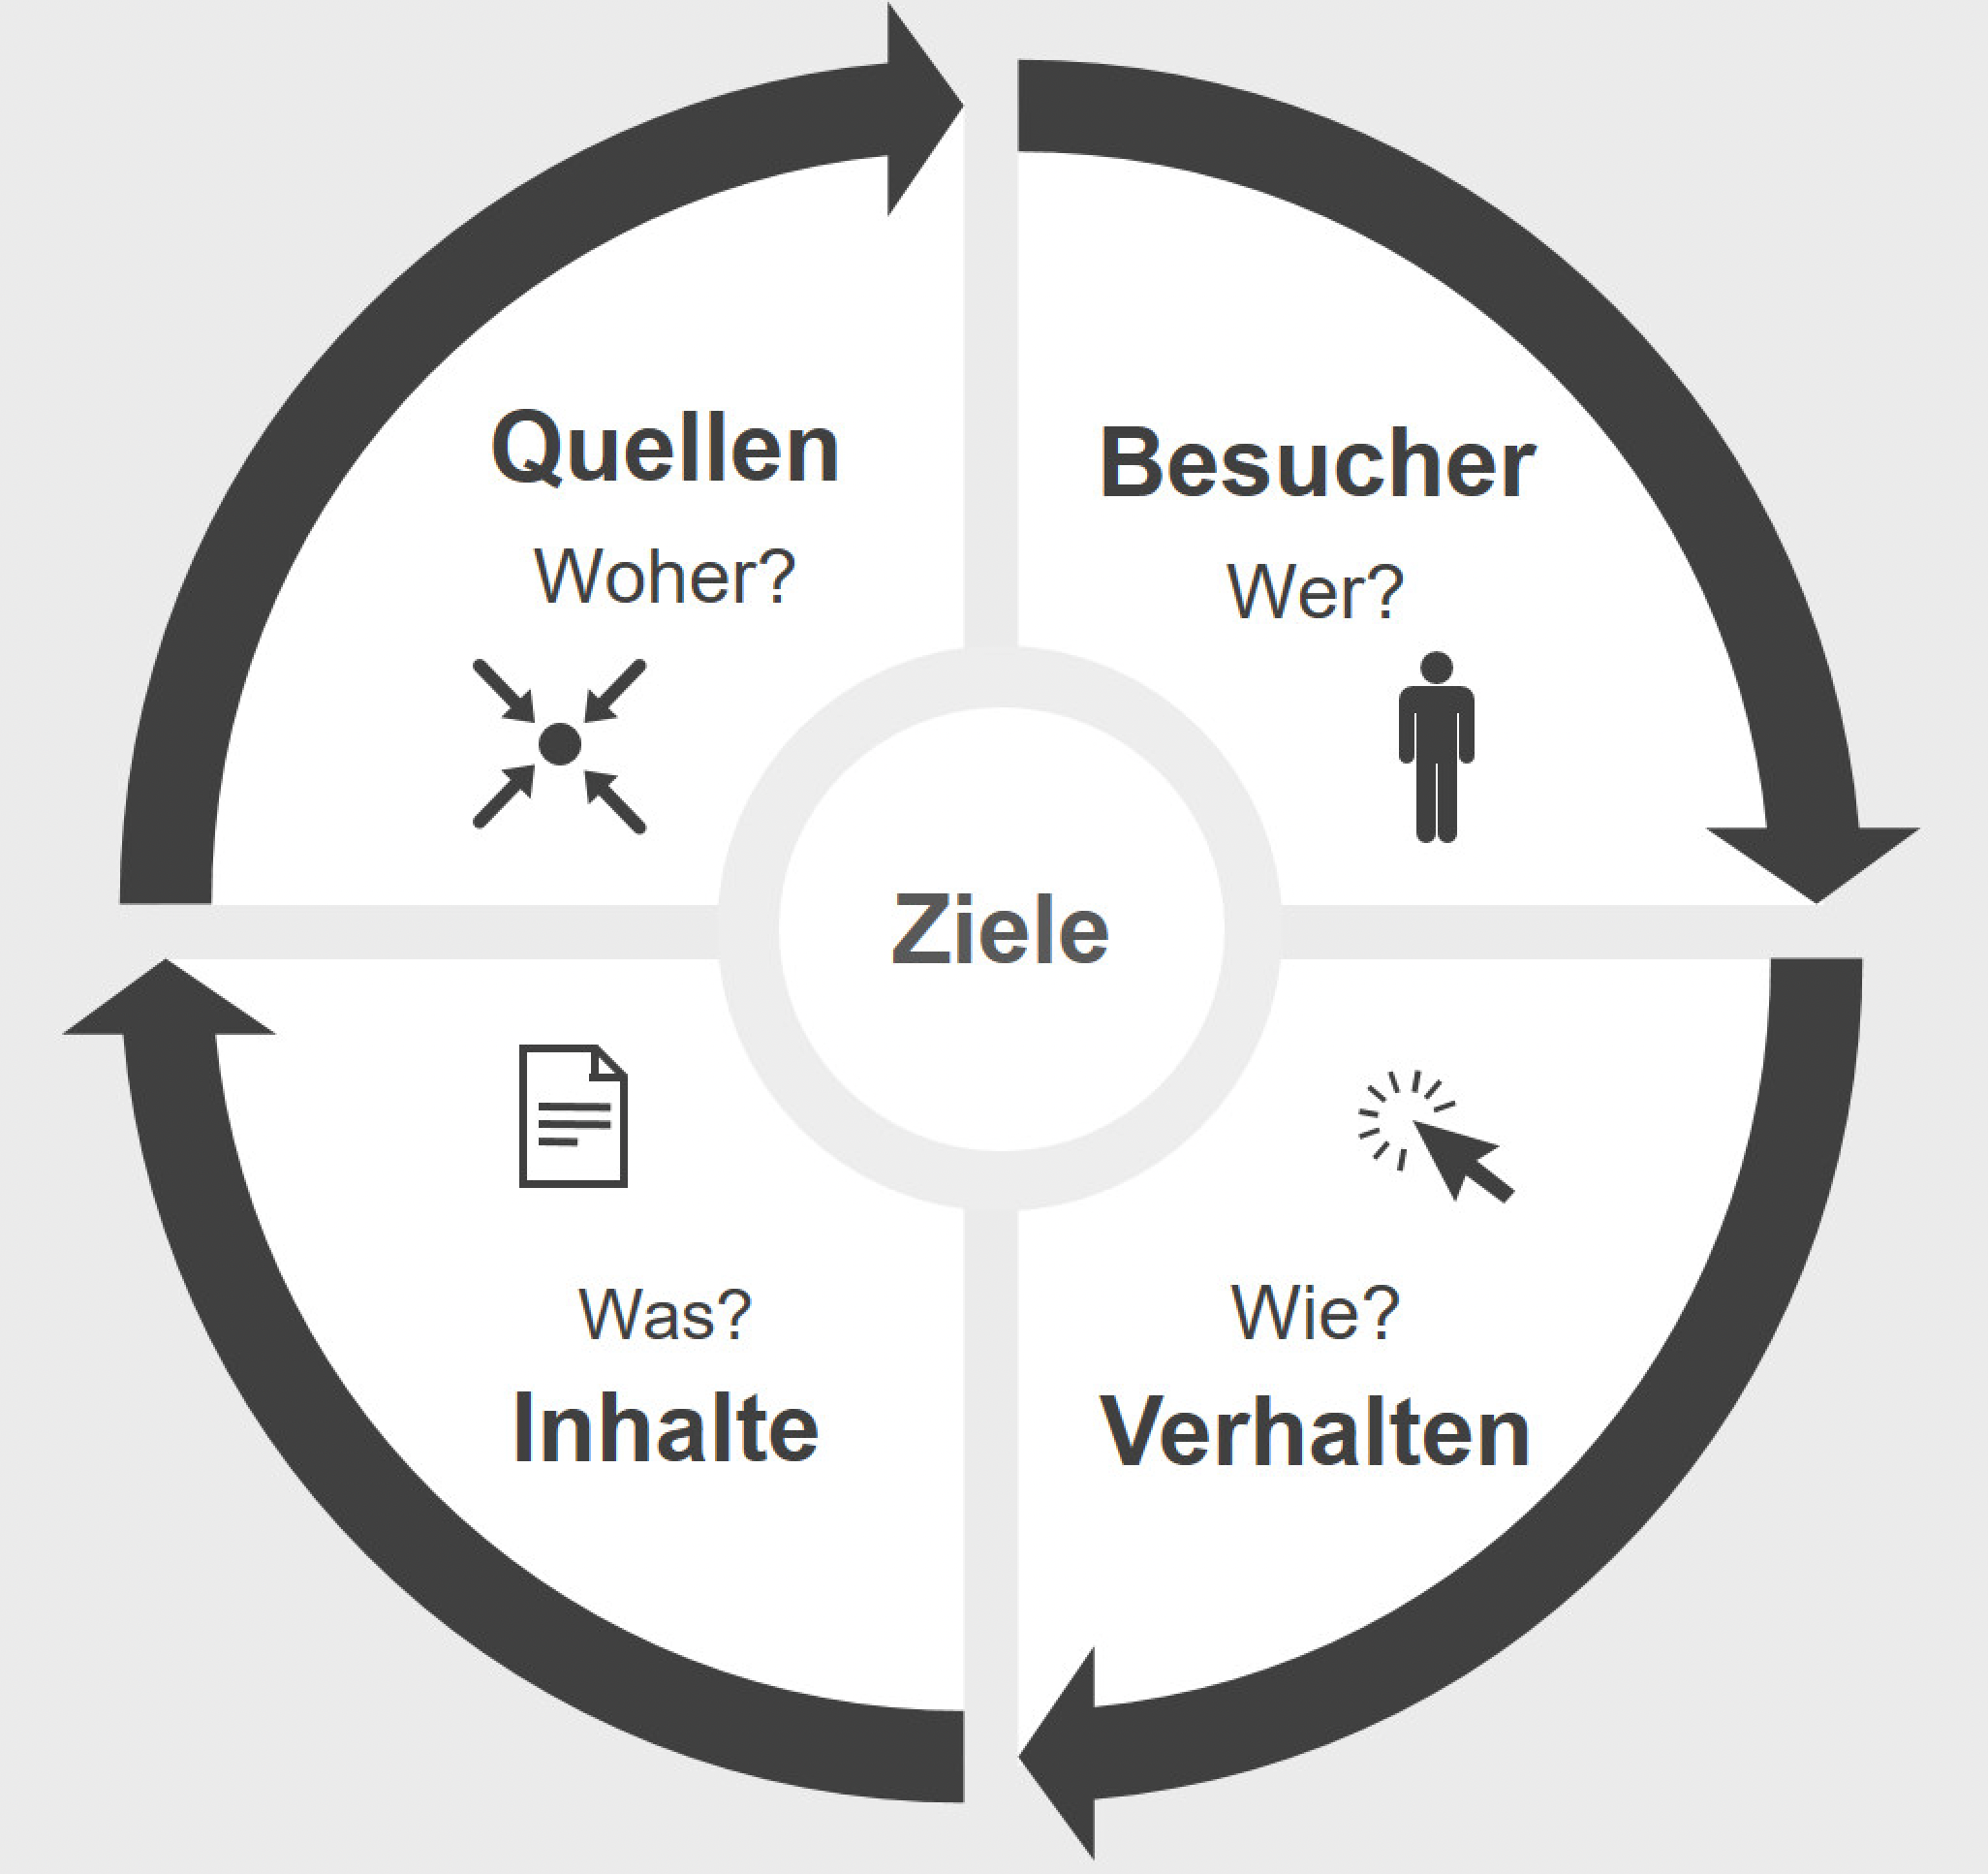
\includegraphics[width=0.5\textwidth]{images/dimensionen.png}%
    \caption{Metriken beleuchten hauptsächlich vier Dimensionen einer Website. [Has19]}%
    \label{fig:dimensionen}%
\end{figure}

Durch die Anordnung der Indikatoren in vier Dimensionen – \textbf{Quellen}, \textbf{Besucher}, \textbf{Inhalte} und \textbf{Verhalten} – wird deutlich, dass die Ziele im Zentrum aus der Analyse der Bereiche abgeleitet werden. Die Zuordnung der KPIs zu den entsprechenden Dimensionen ist in den Tabellen B.1 bis B.6 anahnd der Farbauswahl zu erkennen.

Auf der Dashboardseite \glqq Übersicht\grqq{} bezieht sich die Dimension \textbf{Quellen} auf externe Traffic-Quellen von welchen ein Besucher auf das Bildungsportal gelangt ist. Hierbei soll die Frage: \textit{\glqq Wo kommt denn unser Traffic eigentlich her?\grqq{}} beantwortet werden [Hassler, 2019, Kap.6.2]. Auf den anderen Dashboardseiten wird für diese Dimension die interne Navigation zwischen den einzelnen Webseiten betrachtet. 

Die KPIs aus Tabelle~\ref{tab:kpi_allgemein} werden auf jeder Dashboardseite in der Dimension \textbf{Besucher} angezeigt.

Dimension Verhalten...

Dimension Inhalte...

-> Tabellen einteilen + färben, KPIs besser formulieren, und beschreiben

\section{Visualisierungsmethoden}
%Nachdem die Struktur des Dashboards und die Organisation der %KPIs definiert wurden, stellt sich die Frage, welche %Visualisierungsmethoden am besten geeignet sind, um die %Daten verständlich und aussagekräftig darzustellen.
-> Beschreiben, welche Visualisierungsmethoden geeignet sind für welche Arten von KPIs. Farbdesign + Größe

\section{Grafana als Dashboardtool}
Ebenso wie das Webanalyse-Tool Matomo ist Grafana Open Source und kann sowohl in einer Cloud-Version als auch in einer On-Premise-Version auf einem eigenen Server betrieben werden. Die Selbsthosting-Variante kann unter anderem auf Linux (Debian/Ubuntu), Windows oder macOS installiert werden. Alternativ lässt sich Grafana auch als Docker-Container über ein offizielles Docker-Image bereitstellen. Grafana verwendet standardmäßig eine SQLite-Datenbank, um das Dashboard, die Datenquellen und die Benutzer der Anwendung zu speichern. Für größere Dashboard-Umgebungen, die eine sehr hohe Verfügbarkeit erfordern, kann diese SQLite-Datenbank durch MySQL- oder PostgreSQL-Datenbanken ersetzt werden. Nach der Installation ist Grafana über eine Web-Oberfläche zugänglich, über die Konfigurationen und Dashboards verwaltet werden können. Um diese Web-Oberfläche nutzen zu können, muss JavaScript im Browser aktiviert sein. Unterstützt werden die Browser Chrome, Firefox, Safari und Microsoft Edge. [Grafana Labs, 2025]

\subsection{Datenintegration und Aggregation}
Die Anbindung von Grafana an Matomo, sowie die Aggregation der erfassten Daten kann über diese beiden Varianten erfolgen [De Verteuil, 2022; Matomo, o.D.]:

\begin{enumerate}
    \item \textbf{Anbindung über die Matomo-Datenbank:}  
    Grafana kann direkt mit der Matomo-Datenbank verbunden werden, indem eine entsprechende Datenquelle eingerichtet wird. Durch SQL-Abfragen auf Datenbanktabellen wie \verb|site| oder \verb|log_visit| können KPIs wie Seitenaufrufe, Verweildauer sowie die URL der besuchten Seite extrahiert werden. Außerdem können über die Tabelle \verb|reports| standardisierte und benutzerdefinierte Reports abgerufen werden. In Abbilung~\ref{fig:site} ist die Entität (engl. Entity) \verb|site| mit den zugehörigen Attributen abgebildet. In Abbildung~\ref{fig:report} ist die Struktur der Entity \verb|reports| dargestellt. 
    \item \textbf{Anbindung über die Matomo Reporting API:}  
    Alternativ kann Grafana die Matomo Reporting API (Matomo Analytics API) unter anderem als JSON- oder CSV-Datenquelle nutzen. Dadurch können ebenfalls KPIs und standardisierte Matomo-Reports abgerufen werden, ohne direkt auf die Datenbank zuzugreifen. Diese API ermöglicht es, Reports zu KPIs wie Besucherzahlen, Nutzergeräten, Suchmaschinen, Referrer-Websites, etc. für eine bestimmte Website und einen definierten Zeitraum abzurufen. Das JSON-Format ist hierbei sauberer strukturiert und leichter nachzuvollziehen als CSV, was die Integration und Verarbeitung der Daten vereinfacht. In Abbildung... ist ein solcher Datenexport im JSON-Format dargestellt. -> später eigene Abbildung hierzu einfügen
\end{enumerate}

\begin{figure}[H]
    \centering
    \begin{minipage}{0.48\textwidth}
        \centering
        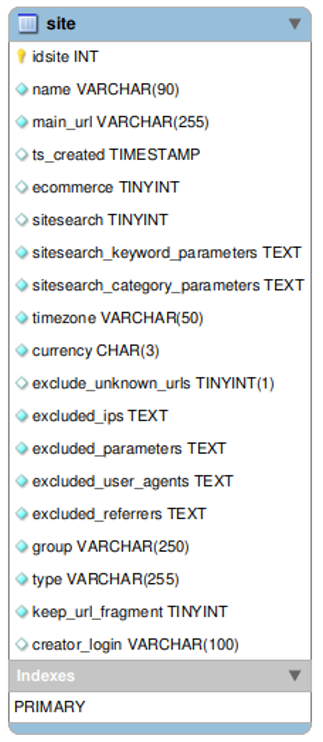
\includegraphics[width=\textwidth]{images/site.png}
        \captionsetup{skip=5pt}
        \caption{Erste Bildbeschreibung.}
        %
        \label{fig:site}
    \end{minipage}
    \hfill
    \begin{minipage}{0.48\textwidth}
        \centering
        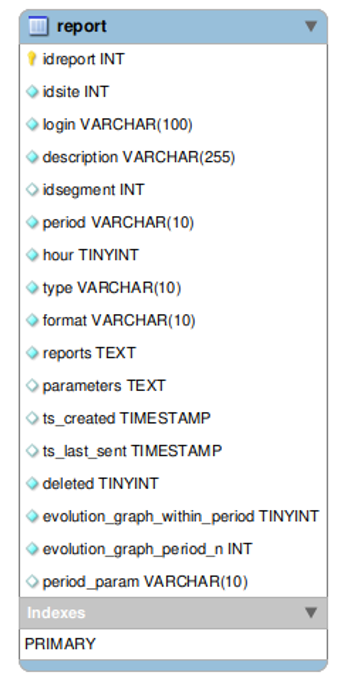
\includegraphics[width=\textwidth]{images/report.png}
        \captionsetup{skip=-1pt}
        \caption{Zweite Bildbeschreibung.}
        %
        \label{fig:report}
    \end{minipage}
\end{figure}

\subsection{Filtermöglichkeiten}
Grafana erlaubt es, alle auf dem Dashboard oder in den einzelnen Panels angezeigten Daten nach Datum, Zeitraum und Benutzergruppen zu filtern. Für die Filterung nach einem bestimmten Zeitbereich kann in Grafana ein Zeitbereichsfilter (engl. Time Range) konfiguriert werden. Hierbei lassen sich sowohl relative Zeiträume (z. B. die letzten fünf Minuten, der letzte Tag oder die letzte Woche) als auch absolute Zeitangaben mit einem exakt definierten Start- und Enddatum festlegen. Die grafische Oberfläche hierfür, der sogenannte Time Picker, ist in Abbildung~\ref{fig:timerange} dargestellt. Auf der linken Seite können absolute Zeitangaben definiert werden. Auf der rechten Seite gibt es eine Auswahl über relative Zeitangaben, wobei hierbei noch zahlreiche weitere verfügbar sind. Im unteren Bereich des Filters ist es außerdem möglich die Zeitzone zu konfigurieren. [Grafana Labs, o.D.]

\begin{figure}[H]
    \centering
    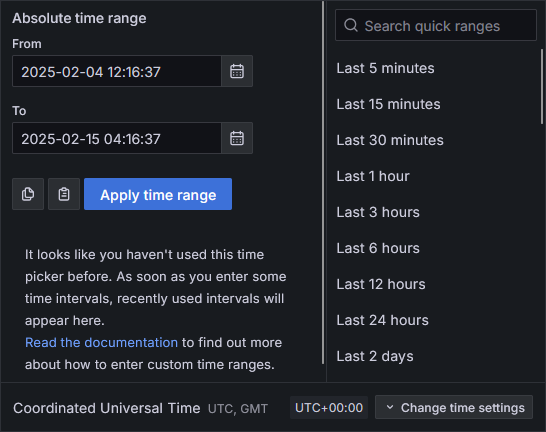
\includegraphics[width=0.5\textwidth]{images/timerange.png}
    %
    \caption{Grafana Time Picker}%
    \label{fig:timerange}%
\end{figure}

Neben der Filterung nach Zeiträumen bietet Grafana auch die Möglichkeit, Daten unter anderem nach Benutzergruppen zu filtern. Hierfür stellt Grafana Variablen bereit, die als dynamische Parameter innerhalb von Abfragen verwendet werden. Eine Variable kann beispielsweise als Query Variable definiert werden und eine SQL-Abfrage ausführen, um nur Daten für eine bestimmte Benutzergruppe, wie Erstbesucher, zu laden. Über ein Dropdwon-Menü können die definierten Variablen ausgewählt werden. Durch diese Auswahl werden nur noch Datensätze aus der Datenbank abgerufen, welche mit dem Wert der Variable übereinstimmen. Die angezeigten Daten auf dem Dashboard werden danach automatisch angepasst. [Grafana Labs, o.D.]

\subsection{Sicherheit und Zugriffskontrolle}
Um sicherzustellen, dass nur authentifizierte Benutzer Zugriff auf das Dashboard haben, sind eine Benutzerauthentifizierung, eine verschlüsselte Verbindung sowie die Absicherung von API- und Datenquellen-Zugriffen erforderlich.

Um den Zugriff auf das Dashboard zu schützen und die Sicherheit der übertragenen Daten zu gewährleisten, stellt Grafana standardmäßig eine integrierte Authentifizierungsfunktion bereit. Bei der ersten Anmeldung wird ein vordefiniertes Admin-Konto mit dem Benutzernamen admin und einem Standardpasswort eingerichtet. Aus Sicherheitsgründen sollte dieses Passwort unmittelbar nach dem ersten Login geändert werden. [Grafana Labs, o.D.]

Außerdem liefert Grafana ein rollenbasiertes Zugriffssystem (RBAC). In der Open Source Version stehen die drei vordefinierte Rollen Viewer, Editor und Admin zur Verfügung. Viewer können Dashboards nur anzeigen, während Editoren zusätzlich Dashboards bearbeiten und neue Panels erstellen dürfen. Administratoren haben vollständigen Zugriff auf alle Konfigurationen innerhalb der Grafana-Instanz. Eine erweiterte rollenbasierte Zugriffskontrolle, die eine feingranulare Berechtigungsverwaltung für Benutzergruppen und API-Zugriffe ermöglicht, ist nur in Grafana Enterprise und Grafana Cloud verfügbar. [Grafana Labs, o.D.]

Um die Sicherheit der Verbindung zu Grafana zu gewährleisten, sollte die Weboberfläche ausschließlich über HTTPS aufgerufen werden. Standardmäßig läuft Grafana über HTTP (Port 3000), jedoch kann eine verschlüsselte HTTPS-Verbindung aktiviert werden, indem in der \texttt{grafana.ini}-Datei entsprechende Konfigurationen vorgenommen werden: \\

\lstinputlisting[caption=Konfiguration der Datei \texttt{grafana.ini} für HTTPS, label={lst:grafanaini}, language=Apache]{listings/grafanaini.txt}

Da das Bildungsportal evaschiffmann.de derzeit auf einem Server gehostet wird, der bereits ein gültiges SSL/TLS-Zertifikat für HTTPS besitzt, muss lediglich die \texttt{grafana.ini} entsprechend angepasst werden, um die sichere Verbindung zu aktivieren. [Grafana Labs, o.D]

Wenn Matomo für HTTPS konfiguriert wurde, ist die Matomo Reporting API ebenfalls über HTTPS erreichbar. Zusätzlich ist für den Zugriff auf die Reporting API ein Authentifizierungs-Token erforderlich, sofern auf private Daten zugegriffen wird. Da Matomo-Statistiken standardmäßig nicht öffentlich zugänglich sind, müssen API-Anfragen einen gültigen Token enthalten. Dieser sollte vertraulich behandelt werden, da er nicht nur den Zugriff auf die API ermöglicht, sondern auch zur Manipulation von Daten genutzt werden könnte. Matomo empfiehlt zudem, den Authentifizierungs-Token ausschließlich für POST-Anfragen zu verwenden und diesen im Request-Body der Anfrage statt als Parameter in der URL zu übergeben, um eine ungewollte Offenlegung, beispielsweise durch das Teilen einer URL, zu vermeiden. [Matomo, o.D.]






